\pdfoutput=1


\documentclass{beamer}
\mode<presentation>
{
%\usetheme{Malmoe}
%\usetheme{Ilmenau}
%\usetheme{Rochester}
%\usetheme{Berkeley}
\usetheme{Madrid}
\setbeamercovered{transparent}
}
\setbeamercolor{normal text}{fg=blue,bg=white}
\setbeamercolor{frametitle}{fg=black,bg=white} 

\usepackage[english]{babel}
\usepackage{lmodern}
%\usepackage[round]{natbib}
%\usepackage[latin1]{inputenc}
%\usepackage{ae} % instead of the following
% three lines if you don't like this look
%\usepackage{mathptmx}
%%
\usepackage{courier}
\usepackage[T1]{fontenc}

\usepackage{multimedia}
%\usepackage{hyperref}

% end BEAMER

% end BEAMER

% LOCAL packages
%\usepackage{dcpic,pictexwd}

\input spheader18.tex

% SLIDE CONTENT
\title{Lazy Stream Programming in Prolog}


\author[P. Tarau \and J. Wielemaker \and T. Schrijvers]{
{\bf Paul Tarau \and Jan Wielemaker \and Tom Schrijvers}\\
~~\\
~~\\
          {\em paul.tarau@unt.edu\\
          J.Wielemaker@vu.nl\\
          tom.schrijvers@cs.kuleuven.be}
}          
   
\date{ICLP'2019, Las Cruces, New Mexico}


\begin{document}

\usebackgroundtemplate{%
 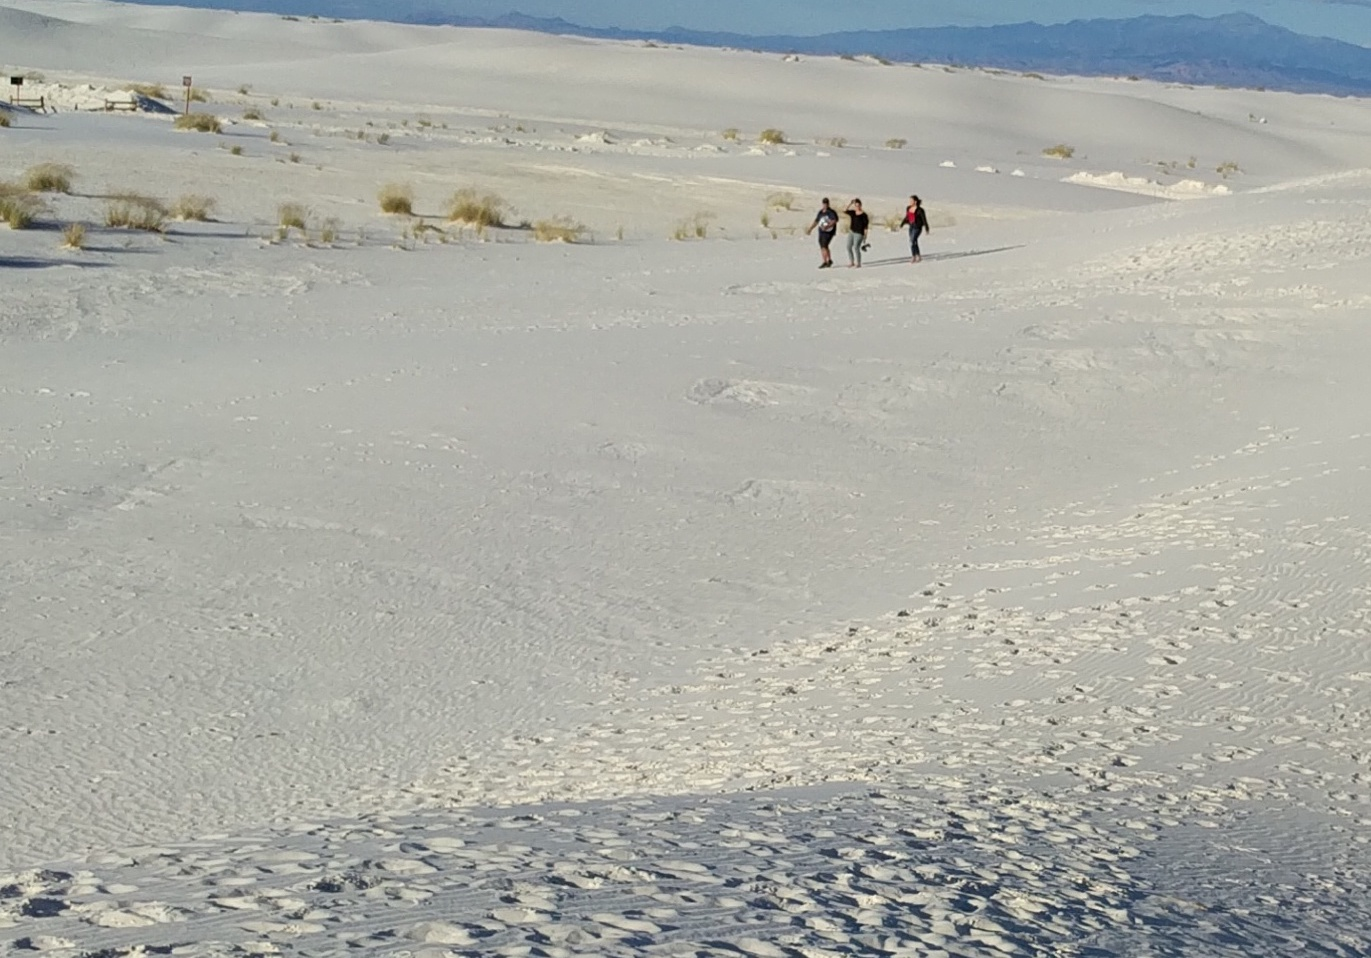
\includegraphics[width=\paperwidth,height=\paperheight]{dunes.jpg}} 
\begin{frame}
\titlepage
\end{frame}
\usebackgroundtemplate{}

%\BFT{Outline}
%\tableofcontents

%\end{frame}





\BFT{Motivation}
\BI
\I \emph{stream processing} is now prevalent in:
Java, Python, C\#, go, Lua, JavaScript etc.

\I processing {\em infinite sequences} is also available in non-strict functional languages like Haskell

\I streams offers a uniform and
(mostly) declarative view on processing finite and infinite sequences

\BI
\I local or network/cloud-based I/O operations
\I large training data sets for machine learning
\I dynamic event streams coming from Web search queries and clicks
\I sensor networks supporting today's IoT infrastructure
\EI
\I $\Rightarrow$ extend Prolog with state-of-the-art lazy
stream processing! 

\EI

\end{frame}




\BFC{Overview}
\BI
\I answer stream generators that 
encapsulate the work of coroutining first-class logic engines
\I support interoperation between forward recursive {\em AND-streams} and backtracking-generated {\em OR-streams}

\I expose them to the application programmer either through an abstract sequence manipulation API or as lazy lists

\I an isomorphism that transports data and  operations between these two representations

\I an algebra of stream generator operations that extends Prolog via an embedded language interpreter providing a compact notation for composition mechanisms

\EI
\end{frame}


\BFT{Contributions}

\BI
\I  simple and clean approach for setting up lazy streams, which
   uniformly encapsulates algorithms, lists, first-class logic engines and other data sources
\I by using attributed variables, we expose lazy streams in the form of lazy Prolog lists
   that, just like conventional lists, can be inspected and decomposed with unification
   
\I an embedded language interpreter supporting an algebra of stream operations
\I we have implemented our approach in several libraries:
   \BE 
   \I \texttt{lazy\_streams}: generator builders, generator operations, an embedded generator algebra interpreter:
    a standalone package at 
   {\small \url{https://github.com/ptarau/AnswerStreamGenerators/raw/master/lazy_streams-0.5.0.zip}}
   \I \texttt{lazy\_lists}:   generator predicates for 
      directly setting up lazy lists (part of SWI-Prolog)
   \I \texttt{pure\_input} library provides a range of predicates for reading
      files and sockets backed by lazy lists (part of SWI-Prolog)
   \EE
%\url{http://www.swi-prolog.org/pldoc/doc/_SWI_/library/lazy_lists.pl},
%\url{http://www.swi-prolog.org/pldoc/doc/_SWI_/library/pure_input.pl}}


\EI

\end{frame}



\BFC{A few use cases}

\BI
\I map operation on infinite streams
\begin{codex}
?- pos(P),neg(N),map(plus,P,N,Zero),show(10,Zero).
[0, 0, 0, 0, 0, 0, 0, 0, 0, 0].
\end{codex}
\I convolution between an infinite and a finite stream
\begin{codex}
?- pos(P),list([a,b,c],L),convolution(P,L,C),show(16,C).
[1-a, 1-b, 2-a, 1-c, 2-b, 3-a, 2-c, 3-b, 4-a, 3-c, 
      4-b, 5-a, 4-c, 5-b, 6-a, 5-c].
\end{codex}

\I evaluating stream expressions
\begin{codex}
?- X in_ [a,b]*(1:4).
X = a-1 ; X = b-1 ; X = b-2 ; X = a-2 ; X = b-3 ; X = a-3 .
\end{codex}
\EI
\end{frame}

\BFC{The stream constructors}
\BI
\I {\em stream generators} are created by a family of constructors, encapsulating sequences
produced algorithmically or as a result of state transformers interfacing
Prolog with the ``outside world''
\I  a design philosophy similar to that of
monads in functional languages
\I a generator is represented 
by a \emph{closure} i.e., a term that can be
called with an additional argument to yield the next element in the stream
\I when the closure has no more elements to yield, it fails
\EI
\begin{tabular}{ccc}
\begin{minipage}{0.4\textwidth}
\begin{code}
ask(E,_):-is_done(E),!,fail.
ask(E,R):-call(E,X),!,R=X.
ask(E,_):-stop(E),fail.
\end{code}
\end{minipage}
&
where
&
\begin{minipage}{0.4\textwidth}
\begin{code}
is_done(E):-arg(1,E,done).
stop(E):-nb_setarg(1,E,done).
\end{code}
\end{minipage}
\end{tabular}
\end{frame}


\BFC{Some basic generators}
\BI
\I an infinite constant stream:
\begin{code}
const(C,=(C)).
\end{code}

\I 
the {\tt rand/1} predicate produces the {\tt random/1} stream generator, which relies on externally maintained state
to yield floating point numbers between 0 and 1
\begin{code}
rand(random).
\end{code}

\I a stream created by incrementally evolving a state:
\begin{code}
gen_next(F,State,X):-
  arg(1,State,X),
  call(F,X,Y),
  nb_setarg(1,State,Y).
\end{code}
\I here {\tt State} acts as a container for destructively updated values using the
{\tt nb\_setarg/3} built-in

\EI
\end{frame}

\BFC{Iterating over the elements of a stream via backtracking}
\BI
\I 
the {\tt in/2} predicate uses {\tt ask/2} to produce the elements on backtracking
\begin{code}
:-op(800,xfx,(in)).

X in Gen:-ask(Gen,A),select_from(Gen,A,X).

select_from(_,X,X).
select_from(Gen,_,X):-X in Gen.
\end{code}

\I with {\tt in/2}, the generator emulates its declarative Prolog equivalent
\I a \alert{declarative} view of a procedural iteration mechanism: it works as if  {\tt member/2} were  used on a list!
\EI
\end{frame}

\BFC{Backtracking with {\tt in/2}}
a stream backed by a list
\begin{codex}
?- list([1,2,3],G),X in G.
G = gen_nextval(list_step, state([2, 3])),
X = 1 ;
G = gen_nextval(list_step, state([3])),
X = 2 ;
G = gen_nextval(list_step, state([])),
X = 3 ;
false.
\end{codex}

elements of a random streams
\begin{codex}
?- rand(G),X in G.
G = random(),
X = 0.7711731055905214 ;
G = random(),
X = 0.32254300867150587 .
\end{codex}
\end{frame}


\usebackgroundtemplate{%
 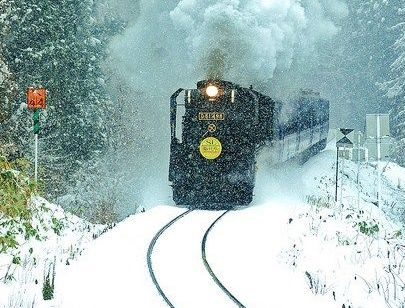
\includegraphics[width=\paperwidth,height=\paperheight]{steameng.jpg}} 
\BFT{A steam {\em engine} pulling a stream of cars (some first class)}

\end{frame}
\usebackgroundtemplate{}


\BFC{First class logic engines}
\BI
\I a first-class logic engine can be seen as a Prolog
virtual machine that has its own stacks and machine state 
\I already present in BinProlog from around {\bf 1995}
\I in their SWI-Prolog implementation, unlike normal Prolog threads
they are
not associated with an operating system thread
\I instead, one asks an engine for
a next answer with the predicate {\tt engine\_next/2}
\I implementing the engine API only assumes that the virtual machine is fully
re-entrant, that it can be queried and that it can stop, yield data and resume
execution as a {\em coroutine}

\EI
\end{frame}

\BFC{Generators built with first class logic engines}
\BI
\I the predicate {\tt eng/3} creates a generator as a wrapper for the {\tt
engine\_next(Engine,Answer)} built-in, encapsulating the answers of that engine
as a stream
\begin{code}
eng(X,Goal,engine_next(Engine)):-
  engine_create(X,Goal,Engine). 
\end{code}

\EI
\end{frame}

\BFC{The AND-stream / OR-stream Duality}
\BI
\I  first-class engines support two ways of producing
a stream of answers
\BI 
\I via backtracking (OR-streams)
\I as part of a
forward moving recursive loop (AND-streams)
\EI
\I the stream generator abstraction makes the user oblivious to this choice of
generation method

\EI
\begin{code}
and_nat_stream(Gen):-eng(_,nat_goal(0),Gen).

nat_goal(N):-succ(N,SN),engine_yield(N),nat_goal(SN).
\end{code}

operationally equivalent to:

\begin{code}
or_nat_stream(Gen):-eng(N, nat_from(0,N), Gen).

nat_from(From,To):- From=To ; succ(From,Next),nat_from(Next,To).
\end{code}

\end{frame}





\BFC{Stream operations: direct sum}
\BI
\I the predicate {\tt sum(+Gen1,+Gen2, -NewGen)} advances by
asking each generator, in turn, for an answer

\begin{code}
sum(E1,E2,sum_next(state(E1,E2))).

sum_next(State,X):-State=state(E1,E2),ask(E1,X),!,
  nb_setarg(1,State,E2),
  nb_setarg(2,State,E1).
sum_next(state(_,E2),X):-ask(E2,X).
\end{code}
\I when one generator terminates, we keep progressing in the other

\I works on finite or infinite streams:
\begin{codex}
?- pos(N),neg(M),sum(N,M,E),show(10,E).
[1,-1,2,-2,3,-3,4,-4,5,-5]
\end{codex}

\EI
\end{frame}

\BFC{Stream operations: direct product, with engines}
\BI
\begin{code}
prod(E1,E2,E):-eng(_,prod_goal(E1,E2),E).
prod_goal(E1,E2):-ask(E1,A),prod_loop(1,A,E1-[],E2-[]).
\end{code}
\I {\tt prod\_loop} runs inside an engine, and returns pairs
\begin{code}
prod_loop(Ord1,A,E1-Xs,E2-Ys):-
  flip(Ord1,Ord2,A,Y,Pair),
  forall(member(Y,Ys),engine_yield(Pair)),
  ask(E2,B),!,
  prod_loop(Ord2,B,E2-Ys,E1-[A|Xs]).
prod_loop(Ord1,_A,E1-_Xs,_E2-Ys):-
  flip(Ord1,_Ord2,X,Y,Pair),
  X in E1, member(Y,Ys), engine_yield(Pair), fail.

flip(1,2,X,Y,X-Y).     flip(2,1,X,Y,Y-X).
\end{code}
\I Example:
\begin{codex}
?- nat(N),nat(M),prod(N,M,R),show(12,R).
[0-0,1-0,1-1,0-1,2-1,2-0,2-2,1-2,0-2,3-2,3-1,3-0]
\end{codex}

\EI
\end{frame}

\BFC{An algebraic view: the embedded Language interpreter}

\begin{center}
\begin{tabular}{rcl@{\hspace{0.4cm}}l@{\hspace{1cm}}cl@{\hspace{0.4cm}}l}
  $F$    & ::=  & $F_1 + F_2$         & \it (sum)         & $\mid$ & $\{F\}$           & \it (setification)\\
         & $\mid$ & $F_1 \times F_2$  & \it (product)     & $\mid$ & $X^G$            & \it (engine) \\
         & $\mid$ & $N:M$             & \it (range)       & $\mid$ & $A$               & \it (constant)\\
         & $\mid$ & $[X|Xs] \mid []$  & \it (list)        & $\mid$ & $E$               & \it (stream)
\end{tabular}
\end{center}

\BI
\I 
the language of stream expressions comprises lists, engines, ranges, constants and existing streams, as well as their sums, products and
\emph{setification} (i.e., removing duplicates)
\I
we have implemented it with a simple interpreter,
the predicate  {\tt eval\_stream(+GeneratorExpression, -Generator)},
which turns a generator expression into a ready-to-use generator that combines 
the effects of its components
\EI
\end{frame}

\BFC{The stream expression evaluator}

\BI
\I
recursing over stream expressions
\begin{code}
eval_stream(E+F,S):- !,
  eval_stream(E,EE),eval_stream(F,EF),sum(EE,EF,S).
eval_stream(E*F,P):- !,
  eval_stream(E,EE),eval_stream(F,EF),prod(EE,EF,P).
eval_stream(E:F,R):- !,range(E,F,R).
eval_stream([],L):-!,list([],L).
eval_stream([X|Xs],L):-!,list([X|Xs],L).
eval_stream({E},SetGen):-!,eval_stream(E,F),setify(F,SetGen).
eval_stream(X^G,E):-!,eng(X,G,E).
eval_stream(A,C):-atomic(A),!,const(A,C).
eval_stream(E,E).
\end{code}

\I the one-liner that trims duplicates, with engines
\begin{code}
setify(E,SE):-eng(X,distinct(X,X in E),SE).
\end{code}
\EI
\end{frame}

\BFC{Backtracking over a stream expression}
\BI
\I we define {\tt in\_/2} as a variant of \texttt{in/2} that takes a 
generator expression rather than a generator
\begin{code}
:-op(800,xfx,(in_)).

X in_ GenExpr:-eval_stream(GenExpr,NewGen),X in NewGen.     
\end{code}

\I Example:
\begin{codex}
?- X in_ ({[a,b,a]}+(1:3)*c).
X = a ; X = 1-c ; X = b ; X = 1-c ; 
X = 2-c; X = 1-c ; X = 2-c ...
\end{codex}

\EI
\end{frame}

\BFC{Lazy Functional Programming constructs: map and reduce}
\BI
\I {\tt map/3} creates a generator that applies a binary predicate
to the subsequent elements in a given stream to produce a new stream
\begin{code}
map(F,Gen,map_next(F,Gen)).

map_next(F,Gen,Y):-ask(Gen,X),call(F,X,Y).
\end{code}

\I note that we do not need to explicitly iterate 
-- like with most other stream operations, we only need to specify a single computation step!
\EI

\BI
\I {\tt reduce(+Closure,+Generator,+InitialVal, -ResultGenerator)}
creates a generator that reduces a finite generator's elements with a closure, 
starting with an initial value
\I  its only element is the resulting single final value
(i.e., like Haskell's {\tt foldl} and {\tt foldr})
\I  used to
generically define arithmetic sums and products over a stream
\EI
\end{frame}

\BFC{Scan: collecting prefix computation results}
\BI
\I {\tt scan(+Closure, +Generator, +InitialVal, -ResultGenerator)}
\I similar to \texttt{reduce/4} but also yields all intermediate results
\I  this is also meaningful for infinite streams
\begin{code}
scan(F,InitVal,Gen,scan_next(state(InitVal),F,Gen)).

scan_next(S,F,Gen,R) :- arg(1,S,X),
  ask(Gen,Y),
  call(F,X,Y,R),
  nb_setarg(1,S,R).
\end{code}
\I the stream of cumulative sums of the natural numbers:
\begin{codex}
?- nat(E), scan(plus,0,E,F), show(11,F).
[0, 1, 3, 6, 10, 15, 21, 28, 36, 45, 55].
\end{codex}

\EI
\end{frame}

\BFC{Stream Wrappers for I/O and Stateful Prolog Features}
\BI
\I we wrap file or socket readers as generators
\I  this has the
advantage that details like opening a file, reading and
closing a stream stay hidden, e.g., as in {\tt term\_reader}:

\begin{code}
term_reader(File,next_term(Stream)):-open(File,read,Stream).

next_term(Stream,Term):-
  read(Stream,X),
  ( X\==end_of_file->Term=X
  ; close(Stream),fail
  ).
\end{code}
\I again, note that we do not need to explicitly iterate
\I we only specify a single step and the end condition
\EI
\end{frame}

\BFC{Lazy Streams as Lazy Lists}
\BI
\I a representation for lazy streams that's familiar to the Prolog user
\I lazy lists look much like regular Prolog lists
\I they can be inspected and deconstructed with unification
\I for instance, DCGs can  be used to parse lazy lists
\EI
\end{frame}

\BFC{Implementing streams as lazy lists}
\BI
\I we delay the
evaluation of a computation until its result is actually needed
\I the lazy list is represented as a
Prolog list where the tail is formed by an attributed variable
\I when inspected through unification,
attributed variables  trigger  the computation and
deliver the actual value

\I building the  list happens incrementally, when needed,
but what has been computed can be reused
\I Example:  the lazy list of natural numbers:
\begin{code}
simple:lazy_nats(List):-simple:lazy_nats_from(0,List). 
simple:lazy_nats_from(N,List):-put_attr(List,simple,N).

simple:attr_unify_hook(N,Value):-succ(N,M),
  simple:lazy_nats_from(M,Tail),Value = [N|Tail].
\end{code}
\EI
\end{frame}

\BFC{The isomorphism:  from/to lazy streams to/from lazy lists}
\BI
\I two predicates witness the isomorphism between the
representations
\I  {\tt
gen2lazy(+Generator,-LazyList)} turns a possibly infinite stream generator into
a lazy list by using the generator as the state on which the lazy list is
based
\I it uses \texttt{ask/2} to advance that state and produce a new element
\begin{code} 
gen2lazy(Gen,Ls):-lazy_list(gen2lazy_forward,Gen,Ls).

gen2lazy_forward(E,E,X):-ask(E,X).
\end{code}
\I the opposite direction is even easier, as the {\tt list/2} generator also works
on lazy lists!
\begin{code}
lazy2gen(Xs, Gen):-list(Xs, Gen).
\end{code}

\EI
\end{frame}

\BFC{Transformers: defining the iso-functor}
\BI
\I 
we can easily transport not just the data representations but also the
operations acting on them
\I  in category theory, this concept is formally known
as an {\em iso-functor}, a mapping that transports morphisms between objects
from one category to another and back

\I the predicate 
{\tt iso\_fun(+Operation, +SourceType, +TargetType, +Arg1, -Result)}
generically transports a predicate of the form {\tt F(+Arg1, -Arg2)} to a domain where
an operation can be performed and brings back the result

\begin{code}
iso_fun(F,From,To,A,B):-call(From,A,X),call(F,X,Y),call(To,Y,B).
\end{code}

\I we have implemented variants for several arities and modes
\EI
\end{frame}

\BFC{Borrowing {\tt map} from lazy steams, for infinite lazy lists}
\BI
\I maplist will loop on lazy lists as its halting condition is unification against the empty list
\I when a list is infinite this never happens
\I we borrow {\tt map} to define a lazy version of {\tt maplist}:
\begin{code}
lazy_maplist(F,LazyXs,LazyYs):-
  iso_fun(map(F),lazy2gen,gen2lazy,LazyXs,LazyYs).
\end{code}
\I Example:
\begin{codex}
?- lazy_nats(Ns),lazy_maplist(succ,Ns,Ps),prefix([A,B,C],Ps).
Ns = [0,1,2|_20314], Ps = [1,2,3|_20332], A=1,B=2,C=3,...
%     ^^^^^                ^^^^^
\end{codex}

\EI
\end{frame}

\BFC{Borrowing {\tt lazy\_sum} form lazy lists}
\BI
\I direct sum proceeds by interleaving elements of the two streams

\begin{code}
sum_(E1,E2, E):-iso_fun(lazy_sum,gen2lazy,lazy2gen,E1,E2, E).

lazy_sum(Xs,Ys,Zs):-lazy_list(lazy_sum_next,Xs-Ys,Zs).
  
lazy_sum_next([X|Xs]-Ys,Ys-Xs,X).
lazy_sum_next(Xs-[Y|Ys],Ys-Xs,Y).
\end{code}
\I a single step of interleaving is expressed declaratively in {\tt lazy\_sum\_next/3}
\EI
\end{frame}

\BFC{Discussion: pros and cons of lazy streams vs. lazy lists}
\BI
\I lazy streams: abstract sequence interface
\I
lazy lists: the concrete list-based view 

\I one can access the $n$-th element of a generator in $O(1)$ space
\I
lazy lists might or might not need $O(n)$ for that, depending on possible garbage collection of their unused prefix
\I
for stream generators no garbage collection is needed when working destructively in constant space

\I their results can be exposed declaratively via the stream algebra

\I lazy lists are reusable, while new generators 
must be created to revisit a sequence

\I $\Rightarrow$ they offer
similar services, but as they interoperate with help of {\tt iso\_fun} predicates,
one can choose the  implementation most suitable for a given algorithm

\EI
\end{frame}

\BFC{Conclusions}
\BI
\I we have described a unified approach to program with finite and infinite stream
generators that enhances Prolog with operations now prevalent in widely used
programming languages like Python, C\#, go, JavaScript, Ruby and Lua
\I our streams support lazy evaluation mechanisms comparable to those in non-strict
functional languages like Haskell

\I as a special instance, we have defined
generators based on first-class logic engines that can encapsulate both
AND-streams and OR-streams of answers
\I  we have provided an embedded
interpreter for our generator algebra to enable declarative expression of
stream algorithms in the form of compact and elegant code

\I we have provided a lazy list representation for our streams, which
interacts nicely with unification and typical Prolog list code and an iso-functor
that supports  transport of operations between lazy lists and generators

\EI
\end{frame}

\usebackgroundtemplate{%
 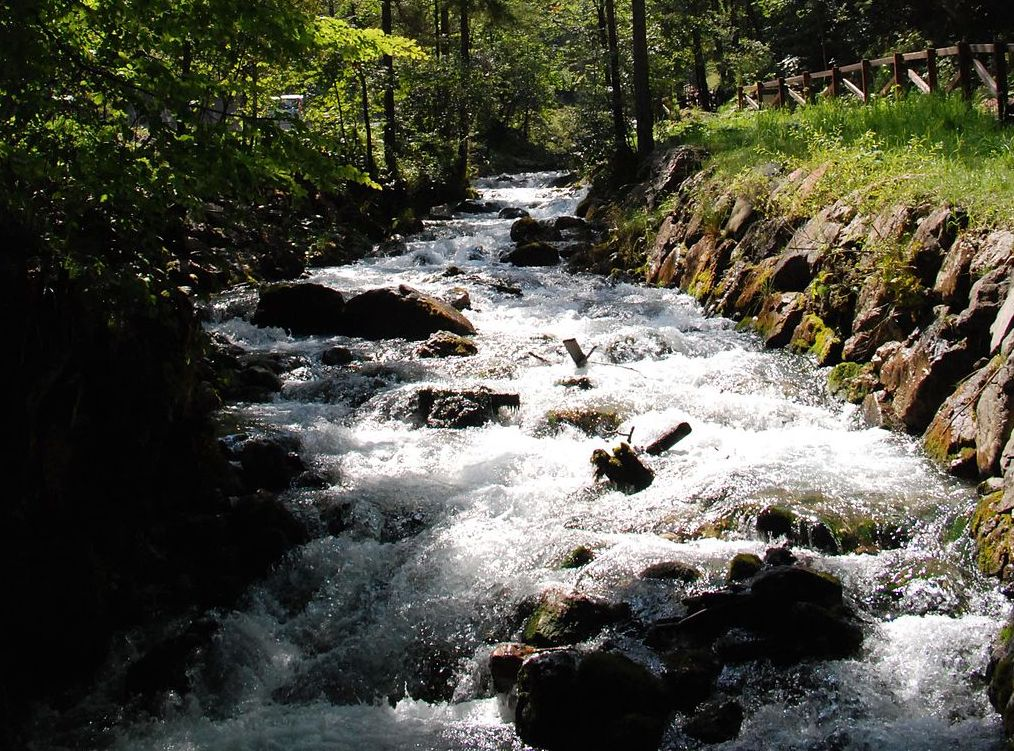
\includegraphics[width=\paperwidth,height=\paperheight]{stream2.jpg}} 

\BFT{~~~~~~~~~~~~~~~~~~~~~~~~~~~~Thank you!}
\begin{center}
{\Huge QUESTIONS?}
\end{center}
%\center{{\tiny Research supported by NSF grant {\bf 1423324}}}

\end{frame}

\usebackgroundtemplate{}
\end{document}